\begin{center}
{\fontsize{15pt}{22pt}\selectfont \textbf{Proposition de correction pour le quizz de statistiques} \par}
\end{center}

\vspace{5mm}

{\fontsize{12pt}{22pt} \textbf{1. Général:}\par}

\vspace{5mm}

1) Que vaut $Cov(X+\mu)$ pour tout $\mu \in \R^p$ déterministe, et tout vecteur aléatoire $X \in \R^p$? \vspace{2mm}

On a:
\begin{lflalign}
& \ Cov(X+\mu) \nonumber \\
= \ & \ \Ex \left[ \left(X+\mu-\Ex(X+\mu) \right) \left(X+\mu-\Ex(X+\mu) \right)^T \right] \nonumber \\
= \ & \ \Ex \left[ \left(X+\mu-\Ex(X)-\mu \right) \left(X+\mu-\Ex(X)-\mu \right)^T \right] \nonumber \\
= \ & \ \Ex \left[ \left(X-\Ex(X) \right) \left(X-\Ex(X) \right)^T \right] \nonumber \\
= \ & \ Cov(X) \nonumber
\end{lflalign} \vspace{1mm}

2) Que vaut $Cov(AX)$, pour toute matrice $A \in \R^{m \times p} $ et tout vecteur aléatoire $X \in \R^p$? \vspace{2mm}

On a:
\begin{lflalign}
\ & \ Cov(AX) \nonumber \\
= \ & \ \Ex \left[ \left(AX-\Ex(AX) \right) \left(AX-\Ex(AX) \right)^T \right] \nonumber \\
= \ & \ \Ex \left[ \left(AX-A\Ex(X) \right) \left(AX-A\Ex(X) \right)^T \right] \nonumber \\
= \ & \ \Ex \left[ \left(A[X-\Ex(X)] \right) \left(A[X-\Ex(X)] \right)^T \right] \nonumber \\
= \ & \ \Ex \left[ A \left([X-\Ex(X)] \right) \left([X-\Ex(X)] \right)^T A^T \right] \nonumber \\
= \ & \ A \Ex \left[ (X-\Ex(X)) (X-\Ex(X))^T \right] A^T \nonumber \\
= \ & \ A \ Cov(X) \ A^T \nonumber
\end{lflalign} \vspace{1mm}

3) Donner un modèle naturel pour ``un lancer de dé'' (non-nécessairement équilibré)? \vspace{2mm}

Un modèle naturel (ou famille de loi naturelle) pour ``un lancer de dé'' est la distribution catégorielle ou multi-Bernoulli, qui généralise la loi Bernoulli à $k$ catégories. Ici, on aura $k=6$, et $\M=\{ \Pb_\theta: \theta \in \R^6 , \ssumm{i=1}{6} \theta_i=1 \}$. \vspace{5mm}

4) Soit $x_1, x_2, \hdots, x_n$ i.i.d. tel que $\Ex [x_1^2]<\infty$. Quel estimateur $\hat{\mu}$ minimise $\ssumm{}{}_{i=1}^n(x_i-\mu)^2$? \\ Donner son biais et sa variance, pour tout $n>1$. \vspace{2mm}

On cherche: $\hat{\mu}=\underset{\mu}{argmin} \ \ssumm{i=1}{n} (x_i-\mu)^2$. La condition de premier ordre est:
\begin{lflalign}
& \ \frac{d}{d \mu} \left(\ssumm{i=1}{n} (x_i-\mu)^2\right)=0 \nonumber \\
\Leftrightarrow \ & \ -2 \ssumm{i=1}{n} (x_i-\mu)=0 \nonumber \\
\Leftrightarrow \ & \ \ssumm{i=1}{n} (x_i-\mu)=0 \nonumber \\
\Leftrightarrow \ & \ \ssumm{i=1}{n} x_i=n \mu \nonumber \\
\Leftrightarrow \ & \ \mu = \frac{1}{n} \ssumm{i=1}{n} \ x_i \nonumber
\end{lflalign}

L'estimateur est donc $\hat{\mu}=\frac{1}{n} \ssumm{i=1}{n} \ x_i$. Son biais est donné par:
\begin{lflalign}
& \ Biais(\hat{\mu}, \mu) \nonumber \\
= \ & \ \Ex_\theta (\hat{\mu}-\mu) \nonumber \\
= \ & \ \Ex_\theta \left( \frac{1}{n} \ \ssumm{i=1}{n} x_i-\mu \right) \nonumber \\
= \ & \ \frac{1}{n} \ \ssumm{i=1}{n} \Ex_\theta (x_i)-\mu \nonumber \\
= \ & \ \frac{1}{n} \ n \Ex_\theta (X)-\mu \hspace{5mm} \text{(car les } x_i \text{ sont identiquement distribuées)} \nonumber \\
= \ & \ \Ex_\theta (X)-\mu \nonumber \\
= \ & \ \mu-\mu \nonumber \\
= \ & \ 0 \nonumber
\end{lflalign}

Sa variance est donnée par:
\begin{lflalign}
& \ var(\hat{\mu}) \nonumber \\
= \ & \ var \left( \frac{1}{n} \ssumm{i=1}{n} x_i \right) \nonumber \\
= \ & \ \frac{1}{n^2} var \left( \ssumm{i=1}{n} x_i \right) \nonumber \\
= \ & \ \frac{1}{n^2} \ \ssumm{i=1}{n} var (x_i) \hspace{5mm} \text{(par indépendence des } x_i \text{)} \nonumber \\
= \ & \ \frac{1}{n^2} \ n \ var (X) \hspace{5mm} \text{(car les } x_i \text{ sont identiquement distribuées)} \nonumber \\
= \ & \ \frac{1}{n} \ var (X) \nonumber
\end{lflalign}

\pagebreak

5) Que vaut le biais de $\frac{1}{n} \ssumm{i=1}{n} (y_i-\bar{y}_n)^2$ ($\bar{y}_n$ est la moyenne empirique) pour des $y_i$ i.i.d. gaussiens, centrés et de variance $\sigma^2$? \vspace{2mm}

On définit la variance empirique comme $\tilde{\sigma}^2=\frac{1}{n} \ssumm{i=1}{n} (y_i-\bar{y}_n)^2$. On peut ensuite la manipuler pour obtenir:
\begin{equation}
\tilde{\sigma}^2=\frac{1}{n} \ssumm{i=1}{n} (y_i-\bar{y}_n)^2 \hspace{3mm} \Leftrightarrow \hspace{3mm} \frac{n}{\sigma^2} \tilde{\sigma}^2 = \ssumm{i=1}{n} \frac{(y_i-\bar{y}_n)}{\sigma^2}^2
\nonumber \end{equation}
Il découle ensuite du théorème de Cochran que:
\begin{equation}
\ssumm{i=1}{n} \frac{(y_i-\bar{y}_n)}{\sigma^2}^2 \sim \chi^2(n-1) \hspace{3mm} \Leftrightarrow \hspace{3mm}  \frac{n}{\sigma^2} \tilde{\sigma}^2 \sim \chi^2(n-1)
\nonumber \end{equation}
Les propriétés de la distribution $\chi^2$ impliquent que $\frac{n}{\sigma^2} \tilde{\sigma}^2$ a une espérance de $(n-1)$ et une variance de $2(n-1)$. On conclut alors:
\begin{equation}
\Ex(\frac{n}{\sigma^2} \tilde{\sigma}^2)=n-1 \ \Leftrightarrow \ \Ex(\tilde{\sigma}^2)=\frac{n-1}{n} \sigma^2
\nonumber \end{equation}
Le biais est donc de:
\begin{equation}
Biais(\tilde{\sigma}^2, \sigma^2)=\Ex(\tilde{\sigma}^2)-\sigma^2=\frac{n-1}{n} \sigma^2-\sigma^2=-\frac{1}{n}\sigma^2
\nonumber \end{equation} \vspace{1mm}

6) On suppose que l'on observe $y_1, \hdots, y_n$, des variables réelles i.i.d., gaussiennes, centrées et de variance $\sigma^2$. Quel est le risque quadratique de l'estimateur $\frac{1}{n} \ssumm{i=1}{n} (y_i-\bar{y}_n)^2$ de $\sigma^2$ ($\bar{y}_n$ est la moyenne empirique)?  \vspace{2mm}

On utilise le même raisonnement qu'à la question précédente, qu'on complète en ajoutant que:
\begin{equation}
var(\frac{n}{\sigma^2} \tilde{\sigma}^2)=2(n-1) \ \Leftrightarrow \ \frac{n^2}{\sigma^4} var(\tilde{\sigma}^2)=2(n-1) \ \Leftrightarrow \ var(\tilde{\sigma}^2) = \frac{2\sigma^4(n-1)}{n^2}
\nonumber \end{equation}
On utilise alors la définition du risque quadratique pour obtenir: \vspace{2mm}
\begin{lflalign}
& \ R(\tilde{\sigma}^2) \nonumber \\
= \ & \ var(\tilde{\sigma}^2)+(biais(\tilde{\sigma}^2))^2 \nonumber \\
= \ & \ \frac{2\sigma^4(n-1)}{n^2}+\frac{\sigma^4}{n^2} \nonumber \\
= \ & \ \frac{\sigma^4(2n-1)}{n^2} \nonumber
\end{lflalign} \vspace{2mm}

7) Quelle est la projection orthogonale du vecteur $\bm{y} \in \R^n$ sur Vect($1_n$), avec $1_n=(1,\hdots,1)^T \in \R^n$? \vspace{2mm}

Soit $\bm{y} \in \R^n$ et $\bm{v}=1_n=(1,\hdots,1)^T \in \R^n$. On considère la projection orthogonale $\bm{w}$ de $\bm{y}$ sur $\bm{v}$, que l'on peut représenter par le grahique suivant:

\begin{figure}[H] \begin{center}
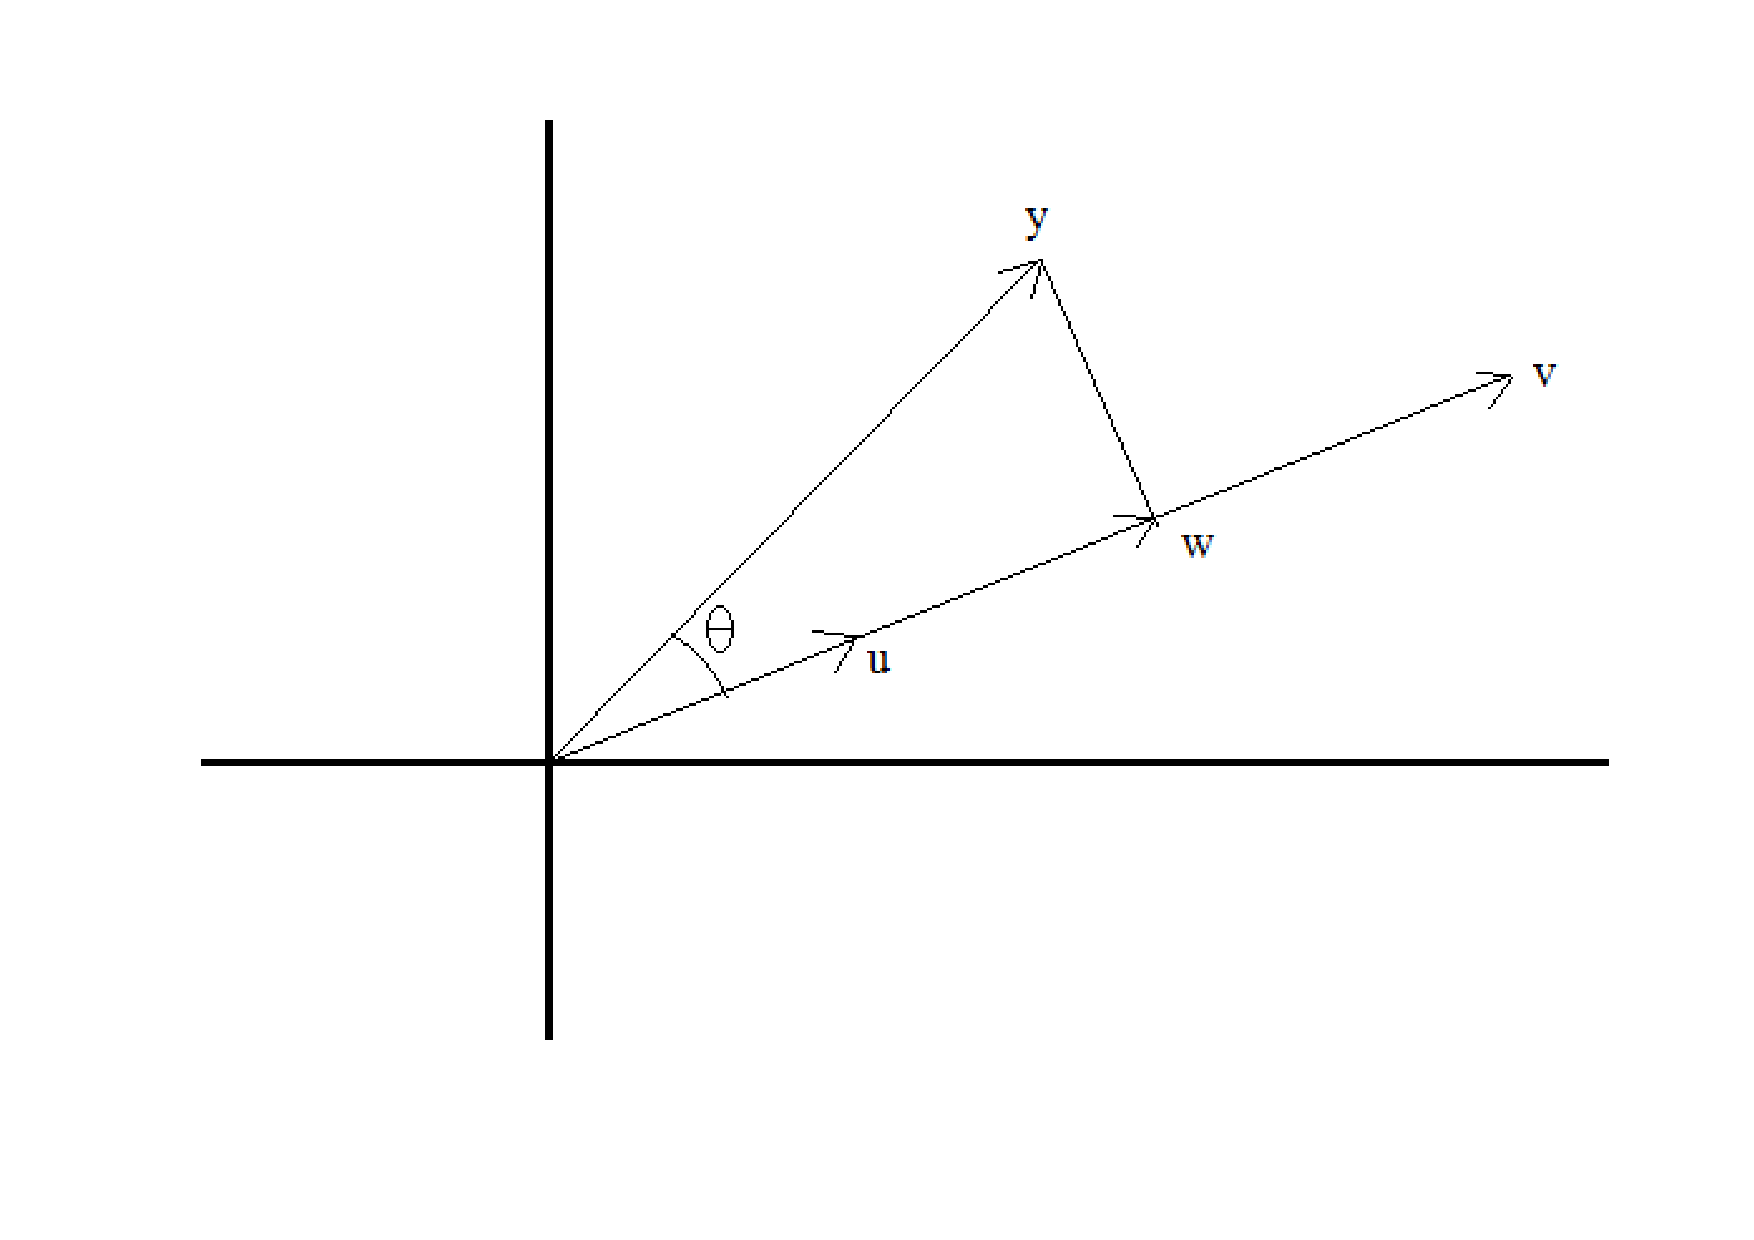
\includegraphics[scale=0.4]{images/graph1.pdf} \vspace{-3mm}
\end{center} \end{figure}

Le vecteur $\bm{u}$ est un vecteur unitaire dans la direction de $\bm{w}$ tel que $u=\frac{1}{\sqrt{n}} 1_n$. On note que par construction $\bm{w}= \|w\| \bm{u}$. Par definition de la fonction cosinus, on a également $cos(\theta)=\frac{\|w\|}{\|y\|}$ et par définition du produit scalaire on a $cos(\theta)=\frac{\langle u,y \rangle}{\|u\| \|y\|}$. En combinant ces deux dernières expressions, on obtient $\|w\|=\langle u,y \rangle $. En substituant dans la première expression, on obtient $w=\langle u,y \rangle \ u$ et donc:
\begin{lflalign}
& \ w \nonumber \\
= \ & \ \langle u,y \rangle \ u \nonumber \\
= \ & \ \langle \frac{1}{\sqrt{n}} 1_n,y \rangle \ \frac{1}{\sqrt{n}} 1_n \nonumber \\
= \ & \ \frac{1}{n} \langle 1_n,y \rangle \ 1_n \nonumber \\
= \ & \ \frac{1}{n} \ (\ssumm{i=1}{n} y_i) \ 1_n \nonumber \\
= \ & \ \bar{y} \ 1_n \nonumber \\
= \ & \ \left( \begin{matrix} \bar{y} \\ \bar{y} \\ \vdots \\ \bar{y} \end{matrix} \right) \nonumber
\end{lflalign} \vspace{2mm}

8) Quels sont les vecteurs $\bm{y} \in \R^n$ tels que $var_n(\bm{y})=0$ ($var_n$ est la variance empirique)?

On obtient que $var_n(\bm{y})=0$ si et seulement si $\frac{1}{n} \ssumm{i=1}{n} (y_i-\bar{y}_n)^2=0$. Celà implique que $y_i=\bar{y} \ \forall i$ (car sinon il existe un $i$ tel que $(y_i-\bar{y}_n)^2>0$ et donc $\ssumm{i=1}{n} (y_i-\bar{y}_n)^2>0$), ce qui n'est possible que si $y_1=y_2=\hdots=y_n=y$, pour $y$ un scalaire donné. On conclut donc que ces vecteurs sont de la forme $\bm{y}=y . 1_n$.












